%%
%% ACM MM Grand Challenge paper draft.
%%

\documentclass[sigconf, screen, review, anonymous]{acmart}

\usepackage{amsmath}
\usepackage{booktabs}
\usepackage{multirow}
\usepackage{tabularx}

\AtBeginDocument{%
  \providecommand\BibTeX{{Bib\TeX}}}

\copyrightyear{2026}
\acmYear{2026}
\setcopyright{none}
\settopmatter{printacmref=false}
\renewcommand\footnotetextcopyrightpermission[1]{}

\acmConference[ACM MM '26]{the 34th ACM International Conference on Multimedia}{November 10--14, 2026}{Rio de Janeiro, Brazil}

\begin{document}

\def\method{\textsc{STEER}}
\title{\method: Domain-Routed Multi-LoRA Teacher On-Policy Distillation for Cross-Domain PCBA Visual QA}

\author{Anonymous Authors}
\affiliation{%
  \institution{Anonymous Institution}
  \country{}}

\renewcommand{\shortauthors}{Anonymous et al.}

\begin{abstract}
The PCBA Standard-to-Real Grand Challenge evaluates multimodal models on a form of industrial visual question answering (VQA) that is difficult for generic vision-language models: a system must transfer manufacturing knowledge from standards-derived examples to cluttered real production imagery, while answering not only perceptual questions but also defect-cause and handling questions. This paper presents \method{}, a domain-routed on-policy distillation framework designed around this cross-domain structure. Instead of training a single model on a naively mixed corpus, \method{} first specializes two homologous LoRA domain teachers: a standard-domain LoRA teacher for rule, cause, and handling knowledge, and a real-world LoRA teacher for high-resolution PCBA perception, template comparison, and dense counting. Since both teachers are lightweight adapters over the same base model, the cost of training multiple teachers is much lower than maintaining independent full checkpoints. A single deployable student is then trained on its own generated trajectories, with each prompt routed to its corresponding domain teacher and dense token-level supervision supplied by teacher prefill probabilities. The on-policy design reduces exposure bias from static teacher completions, while answer-level verifiers keep the optimization aligned with normalized challenge metrics. We use Qwen3.5-9B for controlled ablations and scale the final submission to Qwen3.5-27B. On the official public evaluation, our final system obtains an overall score of 90.920129 and ranks first on the leaderboard.
\end{abstract}

\begin{CCSXML}
<ccs2012>
   <concept>
       <concept_id>10010147.10010178.10010224</concept_id>
       <concept_desc>Computing methodologies~Computer vision</concept_desc>
       <concept_significance>500</concept_significance>
       </concept>
   <concept>
       <concept_id>10010147.10010178.10010179</concept_id>
       <concept_desc>Computing methodologies~Natural language processing</concept_desc>
       <concept_significance>300</concept_significance>
       </concept>
   <concept>
       <concept_id>10010147.10010257.10010293</concept_id>
       <concept_desc>Computing methodologies~Machine learning approaches</concept_desc>
       <concept_significance>300</concept_significance>
       </concept>
</ccs2012>
\end{CCSXML}

\ccsdesc[500]{Computing methodologies~Computer vision}
\ccsdesc[300]{Computing methodologies~Natural language processing}
\ccsdesc[300]{Computing methodologies~Machine learning approaches}

\keywords{industrial visual question answering, PCBA inspection, domain generalization, multimodal large language models, on-policy distillation}

\maketitle

\section{Introduction}
\label{sec:intro}

Industrial inspection is moving from defect localization toward decision support. In printed circuit board assembly (PCBA), an engineer often needs to decide whether a small component is missing, whether a polarized part is mounted correctly, how many pins or components are present, the cause of a soldering defect, and what follow-up action is appropriate. These decisions require both fine-grained visual perception and standards-grounded manufacturing knowledge. Generic multimodal large language models (MLLMs) can describe images fluently, but they are brittle when small objects are densely packed, when the answer depends on package conventions or polarity rules, and when a standard illustration differs sharply from a real factory crop.

The PCBA Standard-to-Real Grand Challenge formalizes this deployment gap as cross-domain VQA for real-world manufacturing inspection~\cite{pcba_challenge_website,pcba_challenge_eval}. The released public data is built from two complementary sources: standards-derived VQA constructed from industrial packaging standards and converted into VQA items, and real-world VQA built from factory production-line imagery~\cite{pcba_challenge_dataset}. The official CodaBench overview and dataset card report a public split with 8,200 training questions and 8,200 test questions, totaling 16,400 questions, covering standard-based knowledge QA, factuality, quantitative reasoning, and attribute reasoning~\cite{pcba_challenge_eval,pcba_challenge_dataset}. Submissions are evaluated on a normalized overall score aggregating accuracy, F1, and bounded counting error~\cite{pcba_challenge_eval}. This setup differs from ordinary industrial anomaly detection: the standard domain contains the rules, causes, and actions; the real domain contains the difficult visual distribution. The winning method therefore has to bridge a semantic domain shift, not only an image-style shift.

Our central claim is that this benchmark should not be treated as a flat instruction-tuning problem. A flat mixture couples two different domains too early: standards questions reward rule recall and conservative action selection, while real-world questions reward local visual discrimination, template comparison, dense counting, and exact normalization. If all examples are simply mixed, the model is encouraged to learn a generic answer style rather than a robust standard-to-real transfer mechanism. Conversely, a pure ensemble is unattractive for a challenge submission because it increases inference cost, complicates answer normalization, and still does not teach one model how to resolve cross-domain conflicts.

We propose \method{}, a domain-routed multi-LoRA-teacher on-policy distillation framework tailored to this challenge. The framework follows a four-stage design. First, a shared MLLM checkpoint is instruction-tuned into a PCBA base model with a canonical prompt and answer protocol. Second, we independently specialize two homologous LoRA teachers from this same base: a \emph{standard-domain teacher} trained on standards-derived VQA, and a \emph{real-world teacher} trained on real production imagery, including factuality, template comparison, counting, and attribute reasoning. Third, the student samples its own responses, and the frozen LoRA teacher matching each prompt domain scores these exact student trajectories by prefill. The student is trained with dense token-level on-policy distillation plus answer-level verifiable objectives. Fourth, deployment uses constrained normalized decoding to map the learned policy onto the official answer space.

The design is inspired by recent multi-teacher on-policy distillation for language-model post-training~\cite{ma2026mopd}, but we adapt the idea to multimodal, metric-normalized, cross-domain industrial VQA. The adaptation is deliberately simple: PCBA VQA has two data domains, so we train two domain teachers and distill them into one student on the student's own sampled trajectories. We instantiate the teachers as LoRA adapters~\cite{hu2021lora}, which makes domain specialization cheap and keeps the teachers naturally homologous because they share the same backbone. The PCBA-specific additions are answer-space canonicalization, visual evidence preservation for the real-world teacher, and constrained normalized decoding for the official answer space.

Our contributions are:
\begin{itemize}
  \item We frame the PCBA Standard-to-Real Challenge as a \emph{two-domain teacher specialization and on-policy distillation} problem, matching the benchmark's construction rather than relying on flat mixed SFT.
  \item We propose \method, a domain-routed multi-LoRA-teacher on-policy distillation method that integrates a standard-domain teacher and a real-world teacher into a single student.
  \item We introduce a lightweight LoRA teacher design that reduces the cost of training multiple domain teachers, together with PCBA-specific components: canonical prompt and answer formatting, released input-format preservation, and answer-level verifiers aligned with accuracy, F1, and normalized MAE.
  \item Our Qwen3.5-27B submission achieves 90.920129 on the official public evaluation and ranks first among public-test submissions; controlled ablations are conducted with Qwen3.5-9B.
\end{itemize}

\section{Related Work}
\label{sec:related}

\paragraph{Industrial anomaly understanding.}
Industrial anomaly detection benchmarks and methods have largely focused on anomaly scoring and localization, including MVTec AD, MVTec LOCO AD, VisA, Real-IAD, PaDiM, PatchCore, DRAEM, CutPaste, and EfficientAD~\cite{bergmann2019mvtec,bergmann2022loco,zou2022visa,wang2024realiad,defard2021padim,roth2022patchcore,zavrtanik2021draem,li2021cutpaste,batzner2024efficientad}. Recent vision-language work extends this setting toward open-ended inspection: WinCLIP and AnomalyGPT adapt large vision-language models to industrial anomalies, while MMAD, MANTA, and UniPCB evaluate defect classification, localization, description, multi-view tiny-object reasoning, and PCB quality inspection~\cite{jeong2023winclip,gu2023anomalygpt,jiang2025mmad,fan2025manta,unipcb2026}. These works provide useful visual priors, but PCBA standard-to-real VQA requires a wider answer space: component identity, defect type, count, cause, and handling decision.

\paragraph{MLLMs and VQA evaluation.}
General MLLMs build on image-text representation learning, visual instruction tuning, and multimodal post-training, as shown by CLIP, Flamingo, BLIP-2, InstructBLIP, LLaVA, LLaVA-NeXT, GPT-4, Gemini, Qwen-VL, InternVL, xGen-MM, and NVILA~\cite{radford2021clip,alayrac2022flamingo,li2023blip2,dai2023instructblip,liu2023llava,Liu24,openai2023gpt4,comanici2025gemini,bai2025qwen25vltechnicalreport,bai2025qwen3,chen2025expandingperformanceboundariesopensource,wang2025internvl35advancingopensourcemultimodal,xue2024xgen,liu2025nvila}. VQA benchmarks have similarly expanded from natural-image QA to bias-controlled, compositional, text-reading, real-user, and expert multimodal reasoning settings~\cite{antol2015vqa,goyal2017making,hudson2019gqa,singh2019textvqa,gurari2018vizwiz,fu2023mme,liu2023mmbench,lu2024mathvista,yue2024mmmu,jiang2025vknowu}. However, these benchmarks rarely combine real manufacturing imagery, exact small-object counting, and standards-derived defect policies in one evaluation.

\paragraph{Knowledge grounding and comparison.}
Standards-derived questions naturally invite retrieval-augmented reasoning: RAG, dense passage retrieval, and retrieval-augmented pretraining can reduce hallucination when answers depend on external definitions or policies~\cite{lewis2020rag,karpukhin2020dense,guu2020realm}. Text retrieval alone is insufficient for PCBA inspection because the model must still decide whether a real crop contains insufficient solder, wrong polarity, or a missing component. \method{} therefore trains a standard-domain teacher for rule knowledge and a real-world teacher for visual evidence, including template comparison and counting.

\paragraph{Domain routing and on-policy distillation.}
Knowledge distillation compresses teacher behavior into a student, with sequence-level and policy distillation extending the idea to generation and decision-making~\cite{hinton2015distilling,kim2016sequence,rusu2016policy}. Preference and RL-based post-training methods such as PPO and DPO further optimize model behavior from sampled outputs or preferences~\cite{schulman2017ppo,rafailov2023direct}. MOPD shows that dense token-level supervision from multiple homologous domain teachers can merge separately trained capabilities more stably than off-policy finetuning or parameter merging~\cite{ma2026mopd}. \method{} follows this principle with two multimodal domain teachers and challenge-metric answer verifiers.

\begin{figure*}[t]
\centering
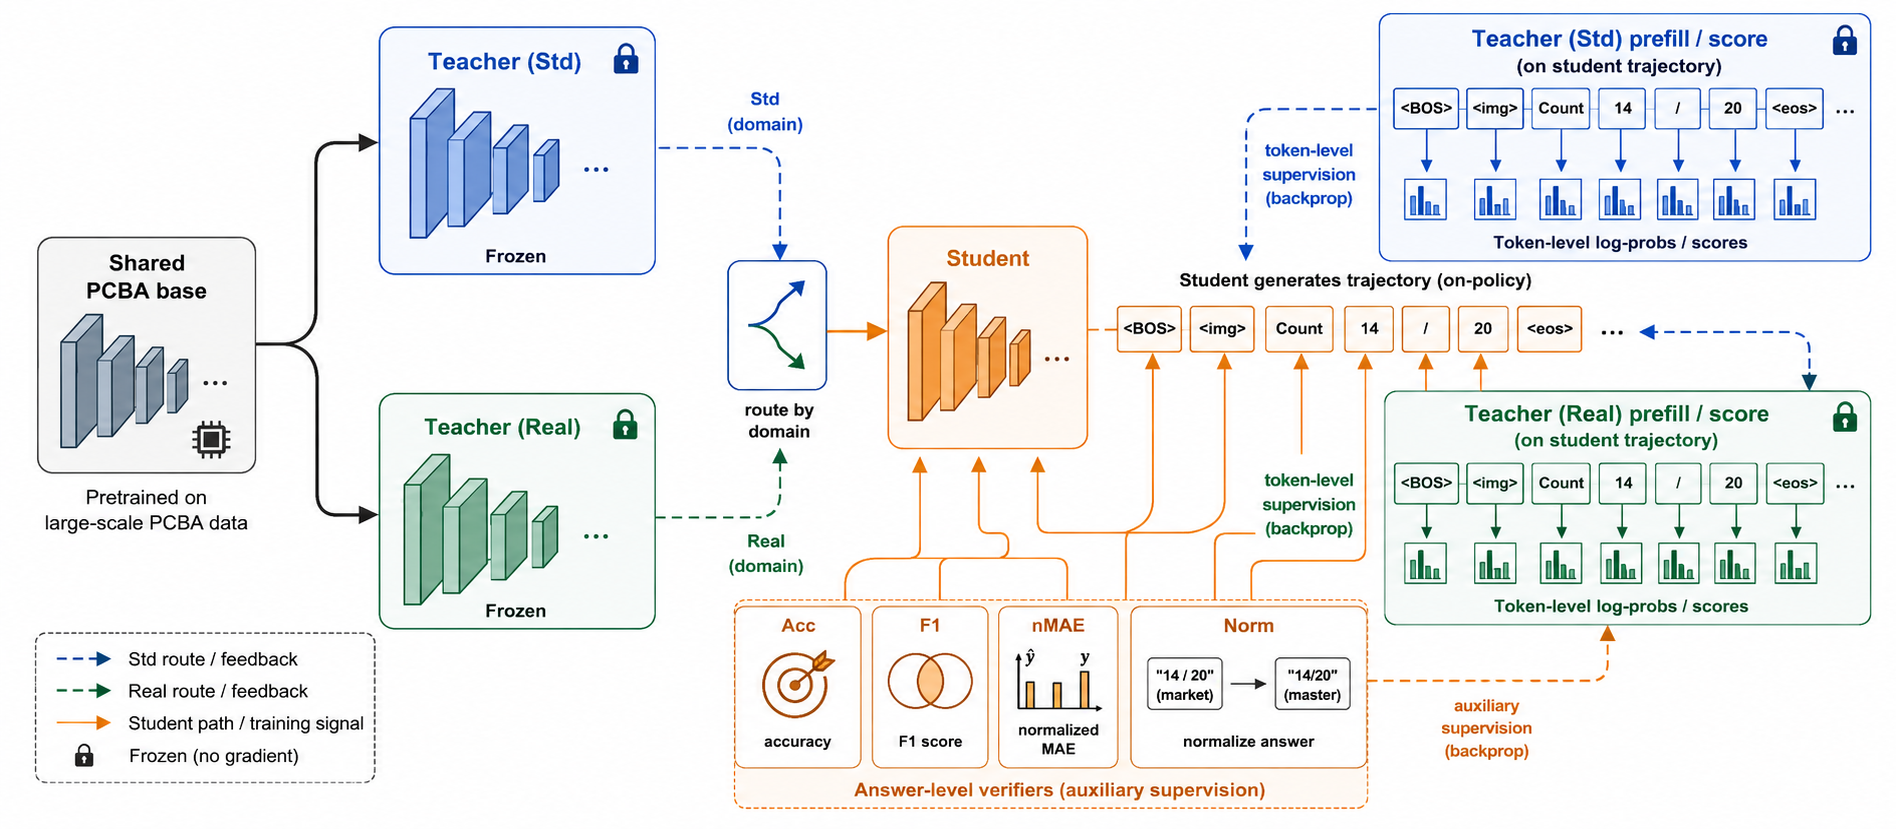
\includegraphics[width=\textwidth]{pic/s2r.png}
\caption{Overview of \method. Standards-derived and real-world PCBA samples are anchored by a shared PCBA base model and specialized into two frozen domain LoRA teachers. During training, the student generates an on-policy answer trajectory; a deterministic domain router selects the matching teacher adapter to prefill and score the same trajectory, providing token-level OPD supervision. Answer-level verifiers normalize task outputs and add metric-aligned auxiliary supervision for accuracy, F1, and normalized-MAE tasks. After distillation, only one deployable student is submitted.}
\Description{Overview figure of STEER, showing standard-derived and real-world PCBA data, a shared PCBA base model, two frozen domain LoRA teachers, domain-routed token-level teacher scoring on student trajectories, answer-level verifiers, and one final student.}
\label{fig:main}
\vspace{-1.2em}
\end{figure*}

\section{Method}
\label{sec:method}

\subsection{Overview}
\label{subsec:overview}

Let each training item be $x=(I, q, m)$, where $I$ is one or more images, $q$ is the question, and $m$ is metadata including question family, input format, candidate options when available, and domain tag when released. The target answer is $a^\star$ after official-style normalization. The model is a conditional policy $\pi_\theta(y \mid x)$ over answer strings. Our goal is to obtain one deployable student that performs well across standards-derived knowledge QA, real-world factuality, quantitative reasoning, and attribute reasoning.

\method{} consists of four components. First, all examples are converted into a canonical PCBA prompt and answer format. Second, two LoRA domain teachers are trained from the same base checkpoint. Third, the student is optimized on its own generated trajectories using the prefill probabilities from the teacher matching each prompt domain. Fourth, inference is constrained by the normalized answer space whenever the question format allows it.

The important design choice is that domains are separated only while producing supervision, not at deployment. A standards question and a real-image question use different teachers during training, but both update the same student policy. At test time, the student has absorbed the two teacher behaviors into a single answer distribution.

The challenge contains multiple input formats. Single-image questions dominate factuality and attribute recognition. Template-target pairs appear when the defect is defined by a deviation from a normal reference, such as missing components or wrong polarity. Some cause and handling questions may include multiple views of the same defect. These are still part of the same real-world domain teacher; they are input-format variations, not separate domains.

\subsection{Canonical Prompt and Answer Space}
\label{subsec:answer_space}

The released training files already provide direct VQA supervision: each item contains image paths, a natural-language question, an optional option dictionary, a short answer, and task metadata when available. We therefore avoid introducing a heavy intermediate label schema. Instead, we canonicalize the interface between the benchmark and the MLLM. Each item is converted into a chat-format example with a PCBA inspection system prompt, one or more image tokens followed by the original question, and an assistant target that is exactly the official short answer.

For multiple-choice questions, the user prompt lists the candidate options and explicitly asks the model to return only the option letter. Binary defect-existence questions are treated as the same two-option case. For quantitative questions, where no option dictionary is provided, the prompt asks for a number only and the assistant target is the integer answer string. This protocol matches the public data format and makes answer normalization part of training rather than only a post-processing step.

\paragraph{Task metadata.}
Domain, task family, and input-format metadata are used for routing, batching, and analysis, not as fields that the model must generate. Standard-derived samples are routed to the standard-domain teacher; real-world samples are routed to the real-world teacher. Task labels such as component type, defect type, mount side, and counting are used to balance batches and to attach the appropriate verifier, while the supervised output remains the same short answer used by the official submission.

\paragraph{Output normalization.}
The final-answer loss is applied to the normalized answer span. For option questions, valid outputs are restricted to the provided option keys; for numeric questions, the first valid integer is extracted and compared with the reference count. At inference time the same normalization maps free-form model text back to a submission-friendly answer. This keeps the method faithful to the released data while reducing avoidable metric loss from verbose generations, spelling variants, or extra units.

\subsection{Multi-LoRA Domain Teachers}
\label{subsec:teachers}

\paragraph{Parameterization.}
Let $\theta_0$ denote the shared PCBA base model. Instead of training two full teacher checkpoints, we instantiate each domain teacher as a LoRA adapter on top of $\theta_0$~\cite{hu2021lora}. For a linear projection $W$ in the adapted modules, domain $d\in\{\mathrm{std},\mathrm{real}\}$ uses
\begin{equation}
W^{(d)} = W + \frac{\alpha}{r} B^{(d)} A^{(d)},
\label{eq:lora}
\end{equation}
where $A^{(d)}$ and $B^{(d)}$ are trainable low-rank matrices, $r$ is the adapter rank, and $\alpha$ is the LoRA scaling factor. The frozen teacher policy for domain $d$ is therefore $\pi_{\phi_d}=\pi_{\theta_0,\Delta_d}$, where $\Delta_d$ denotes the LoRA adapter. This design reduces both training and serving cost for multiple teachers: the memory-heavy backbone weights are shared, while each domain expert is represented by a small adapter.

\paragraph{Memory-efficient multi-LoRA serving.}
The LoRA parameterization lets us serve two teachers without loading two full MLLM replicas. During OPD training, we run one frozen base teacher server for $\theta_0$ and mount both domain adapters, $\Delta_{\mathrm{std}}$ and $\Delta_{\mathrm{real}}$, on the same service. A teacher prefill request contains the prompt, the student trajectory, and an adapter identifier derived from the sample domain. The server activates the requested LoRA adapter and returns token log-probabilities under the corresponding domain teacher. This makes multi-teacher OPD practical under a fixed GPU memory budget: the base model is resident once, and adding a new domain teacher mainly adds LoRA weights rather than another copy of the vision-language backbone. Thus, our multi-teacher design is implemented as domain-routed adapter selection on a shared teacher backbone, not as two independent full-model services.

\paragraph{Standard-domain teacher.}
The standard-domain teacher $\pi_{\phi_{\mathrm{std}}}$ is optimized on standards-derived VQA, defect definitions, cause analysis, and handling decisions. Its role is to encode normative knowledge: which defects are unacceptable, what likely process causes are associated with each defect, and what action should follow. When allowed by the competition rules, a retrieval index over permitted standards-derived notes is used during teacher training to expose the model to concise rule snippets. The distilled student does not need retrieval at inference, but it inherits the teacher's standards-grounded answer distribution.

\paragraph{Real-world teacher.}
The real-world teacher $\pi_{\phi_{\mathrm{real}}}$ is optimized for released real PCBA image inputs. It keeps the original input structure of each sample, including single-image questions, multi-image questions, mount-side views, and template-target pairs when they are provided by the benchmark. Its objective covers defect existence, defect type, component recognition, mount side, attribute reasoning, component counting, and pin/lead counting. Template comparison and counting are handled as real-domain training formats rather than separate teachers. The goal is to make the teacher's token probabilities sensitive to visual cues under real factory variation without relying on a separate augmentation pipeline.

Together, the two LoRA teachers match the two data domains of the challenge. The standard-domain teacher specializes in rule and action knowledge; the real-world teacher specializes in visual recognition, comparison, and counting. This division is used only during training; the final submission remains a single student model.

\paragraph{Homologous initialization.}
All teachers are initialized from the same PCBA base checkpoint as the student, and only their LoRA adapters are specialized. This choice follows the stability observation in multi-teacher on-policy distillation: teachers that are behaviorally close to the student provide useful dense gradients, while distributionally distant teachers can destabilize on-policy learning~\cite{ma2026mopd}. In our setting, sharing the backbone makes this homology explicit and keeps answer format and domain terminology aligned.

\subsection{Domain Routing}
\label{subsec:routing}

For each prompt $x$, a deterministic domain function $d(x)\in\{\mathrm{std},\mathrm{real}\}$ selects the teacher. Standards-derived questions are routed to $\pi_{\phi_{\mathrm{std}}}$; real-world questions are routed to $\pi_{\phi_{\mathrm{real}}}$. In implementation this domain id selects the corresponding LoRA adapter in the shared teacher server. This is the same prompt-to-domain routing used in MOPD: the route determines which frozen domain teacher scores the student's sampled trajectory. The router is not a learned module and is not used at inference time, because the final model is the distilled student.

\subsection{Domain-Routed On-Policy Distillation}
\label{subsec:opd}

On-policy distillation differs from ordinary teacher-forced distillation in the distribution on which the teacher is queried. In off-policy SFT, the student imitates teacher-written completions and therefore only observes prefixes produced by the teacher or by the dataset. In OPD, the student first samples its own response from the current policy:
\[
y=(y_1,\ldots,y_T), \qquad
y \sim \pi_\theta(\cdot \mid x).
\]
The selected LoRA teacher $\pi_{\phi_{d(x)}}$ then prefills this same trajectory, yielding token probabilities $\pi_{\phi_{d(x)}}(\cdot \mid x,y_{<t})$ under the student's prefixes. The teacher is not asked to generate an alternative answer; it only scores the states that the student actually visits. This converts each sampled trajectory into dense token-level feedback and avoids exposure bias from static teacher completions.

Formally, OPD minimizes reverse KL from the student to the routed teacher along the student's own state distribution:
\begin{equation}
\mathcal{L}_{\mathrm{opd}} =
\mathbb{E}_{x,y\sim\pi_\theta}
\left[
\frac{1}{T}\sum_{t=1}^{T}
D_{\mathrm{KL}}\left(
\pi_\theta(\cdot\mid x,y_{<t}) \;\middle\|\;
\pi_{\phi_{d(x)}}(\cdot\mid x,y_{<t})
\right)
\right].
\label{eq:opd}
\end{equation}
Following the policy-gradient instantiation of MOPD, we optimize Eq.~\ref{eq:opd} through a sampled-token estimator. The gradient of the reverse-KL objective can be written as a policy-gradient update where the token-level teacher-student log-probability gap acts as the advantage:
\begin{align}
A_t =
\operatorname{sg}\left[
\log \pi_{\phi_{d(x)}}(y_t\mid x,y_{<t})
- \log \pi_\theta(y_t\mid x,y_{<t})
\right], \label{eq:advantage}\\
\mathcal{L}_{\mathrm{pg}} =
-\mathbb{E}\left[
\frac{1}{T}\sum_t \operatorname{clip}(A_t,-A_{\max},A_{\max})
\log \pi_\theta(y_t\mid x,y_{<t})
\right].
\label{eq:pg}
\end{align}
Here $\operatorname{sg}$ stops gradients through the advantage, and clipping prevents rare low-probability tokens from dominating the update. We use this policy-gradient form directly rather than a top-$k$ distillation variant. Recent work~\cite{ma2026mopd} reports that when teachers and students are homologous, policy-gradient and top-$k$ losses have similarly stable trajectories, with the policy-gradient variant slightly stronger in the comparison; the same analysis finds that top-$k$ does not add stability under homologous teachers and can be less stable under a distributionally mismatched teacher. Our setting is intentionally homologous: the two teachers and the student share the same PCBA base model, and the teachers differ only by LoRA adapters. The simpler policy-gradient objective is therefore the appropriate instantiation for \method{}.

\paragraph{On-policy supervision under student prefixes.}
Static teacher completions are brittle for this benchmark because the same visual evidence can be verbalized in many ways while the official answer may be a short normalized token. If the student is trained only on teacher-written rationales, it may learn a teacher style but still fail when its own partial generation drifts into a different wording. On-policy distillation scores the student's actual prefix, so the teacher signal remains meaningful after such drift. This is particularly useful for numeric questions, where an early wording error should not force the rest of the trajectory to imitate an irrelevant teacher completion.

\paragraph{Two-domain teacher specialization.}
The challenge has two data domains, not three. Counting, template comparison, and attribute recognition are difficult subskills, but they are learned inside the real-world teacher because their supervision comes from real production imagery. Keeping the teacher set at two makes the method match the benchmark design and keeps the distillation stage close to MOPD: sample with the student, route by domain, prefill with the corresponding frozen LoRA teacher, and update the student with dense token-level supervision.

\subsection{Answer-Level Verifiers}
\label{subsec:verifiers}

Token-level distillation alone may copy a teacher's style without improving the exact metric. We therefore add answer-level verifiers aligned with the official normalization. For multiple-choice and binary questions, the verifier reward is exact match after normalization. For counting, the reward is a bounded linear score:
\begin{equation}
R_{\mathrm{count}}(\hat{n},n^\star)=
1-\min\left(\frac{|\hat{n}-n^\star|}{\rho},1\right),
\label{eq:count_reward}
\end{equation}
where $\rho$ is a family-specific range chosen on the training split. The final training objective combines on-policy distillation, supervised answer likelihood, and verifier optimization:
\begin{equation}
\mathcal{L} =
\mathcal{L}_{\mathrm{pg}}
+\lambda_{\mathrm{ans}}\mathcal{L}_{\mathrm{ans}}
-\lambda_{\mathrm{ver}}\mathbb{E}[R_{\mathrm{ver}}].
\label{eq:final_loss}
\end{equation}
The supervised term $\mathcal{L}_{\mathrm{ans}}$ is computed only on the normalized final answer span, preventing the model from overfitting to long rationales. During distillation, rationales are used as hidden scaffolding; during submission, only the final answer is emitted.

For multiple-choice questions, the verifier evaluates the option after answer normalization, not the free-form rationale. For defect existence, we maintain a balanced replay buffer so that positive/negative supervision does not collapse to the dominant class. For counting, the verifier is intentionally smooth: an answer off by one should be penalized less than a completely implausible count during training, even though the official accuracy component may be exact. This smooth reward improves sample efficiency while preserving exact-integer supervision on the normalized answer span.

\subsection{Standards-to-Real Curriculum}
\label{subsec:curriculum}

We use a curriculum that mirrors the benchmark's intended transfer direction. The first phase trains the PCBA base model on the canonical prompt and answer protocol across all public training questions. The second phase trains the standard-domain and real-world LoRA teachers independently with domain-specific data. The third phase performs \method{} domain-routed distillation with mixed-domain batches. In the fourth phase, we run short verifier tuning on normalized answer spans.

Concretely, the pipeline starts with prompt and answer canonicalization, including option formatting, numeric-answer formatting, family and input-format metadata, and the original image or template views provided by each sample. It then trains a shared PCBA base policy, specializes two LoRA teachers from that base, freezes the teachers during domain-routed on-policy distillation, and finishes with metric tuning for option scoring, numeric answer normalization, and answer-span likelihood. Because each stage has a clear output, either domain adapter can be retrained and distilled again without restarting the full recipe.

The curriculum preserves the released input structure rather than introducing additional augmentation. Single-image, multi-image, and template-target examples are kept in their original formats, while only the prompt wrapper and answer format are canonicalized. Standards-derived samples keep their original question and option wording, which preserves the standard-derived taxonomy while presenting the answer through the same short-output protocol as real-world samples. This keeps the standard-to-real transfer claim tied to domain-routed supervision rather than to extra image preprocessing.

\vspace{-0.3em}

\section{Design Rationale}
\label{sec:rationale}

\paragraph{Benchmark-driven decomposition.}
The key design choice is to preserve the benchmark's two-domain asymmetry. Standards-derived items are not merely extra training samples; they carry normative semantics about defect definitions, causes, and handling. Real images are not merely noisier versions of the same samples; they expose the visual state under clutter, lighting variation, dense component layouts, template comparisons, and exact counting requirements. Flat SFT collapses these signals into one average answer style, making it easy to memorize that a defect name implies a handling action while failing to verify that the defect is actually present. \method{} keeps the domains commensurable through a shared prompt and answer protocol, but specializes one teacher per domain before distilling them into one student.

\paragraph{Behavior-space distillation.}
Retrieval, inference-time ensembling, and parameter merging each solve only part of the problem. Retrieval supplies rules but cannot inspect polarity marks or solder joints. Ensembling preserves domain experts but increases cost and multiplies answer formats. Weight merging mixes checkpoints that have deliberately learned different domain priors. Domain-routed on-policy distillation instead treats the two teachers as training instruments: standards knowledge and real-image perception supervise the student's own trajectories. The final system therefore internalizes standard-to-real transfer as one deployable policy, without carrying a router, an ensemble, or an external rule engine at inference time.

\paragraph{LoRA-based teacher specialization.}
MOPD is attractive because teachers can be developed independently, but training and storing full MLLM teachers for every domain is expensive. Our two-domain setting is small enough to be practical, yet LoRA makes the design cleaner: both teachers share the same base model and differ only by domain adapters. This preserves the homologous-teacher assumption in MOPD, reduces GPU memory and checkpoint storage, and allows rapid iteration on one domain without perturbing the other. During distillation, the teacher prefill service only needs to activate the standard or real LoRA adapter; after distillation, the submitted model is still a single student rather than a runtime adapter ensemble.

\vspace{-0.3em}

\begin{table*}[t]
\centering
\caption{Official public evaluation breakdown of our final Qwen3.5-27B submission. Overall score is the weighted sum of task-level normalized metrics using task proportions as weights: 90.920129.}
\vspace{-1.0em}
\label{tab:main_results}
\def\mainresultscale{0.8} % Adjust this value to scale the table width.
\footnotesize
\setlength{\tabcolsep}{3.5pt}
\renewcommand{\arraystretch}{1.02}
\resizebox{\mainresultscale\textwidth}{!}{%
\begin{tabular}{llrrrrl}
\toprule
Task & Metric & Count & Weight & Score & Contribution & Details \\
\midrule
standard\_knowledge & Acc. & 1600 & 0.195122 & 0.735625 & 0.143537 & 1177/1600, inv=0 \\
component\_type & Acc. & 1000 & 0.121951 & 0.950000 & 0.115854 & 950/1000, inv=0 \\
mount\_side & Acc. & 400 & 0.048780 & 0.965000 & 0.047073 & 386/400, inv=0 \\
defect\_existence & F1 & 2000 & 0.243902 & 0.976148 & 0.238085 & TP/FP/FN/TN=1105/30/24/841 \\
defect\_type & Acc. & 2000 & 0.243902 & 0.900500 & 0.219634 & 1801/2000, inv=0 \\
count\_component & nMAE & 400 & 0.048780 & 0.982192 & 0.047912 & MAE=2.4575, R=138 \\
count\_pin\_lead & nMAE & 400 & 0.048780 & 0.990692 & 0.048326 & MAE=2.42, R=260 \\
attribute\_reasoning & Acc. & 400 & 0.048780 & 1.000000 & 0.048780 & 400/400, inv=0 \\
\bottomrule
\end{tabular}
}
\vspace{-0.9em}
\end{table*}

\section{Experiments}
\label{sec:experiments}

\subsection{Dataset and Evaluation}
\label{subsec:dataset}

We evaluate on the PCBA Standard-to-Real Grand Challenge. The official CodaBench overview and dataset card report a released public split of 16,400 questions, with 8,200 training questions and 8,200 test questions~\cite{pcba_challenge_eval,pcba_challenge_dataset}. The dataset includes standards-derived VQA and real-world production-line VQA~\cite{pcba_challenge_dataset}. The question families are standard-based knowledge QA, factuality, quantitative reasoning, and attribute reasoning. The official platform reports a normalized overall score using accuracy for single-choice questions, F1 for defect existence, and bounded normalized MAE for counting~\cite{pcba_challenge_eval}.

There are two evaluation settings in this paper. For the final challenge submission, we train on the released training set, generate answers for the unlabeled public test set, and report the score returned by the official leaderboard. For post-challenge controlled ablations, the public test labels are not available. We therefore create a fixed 8:2 split from the released 8,200-question training set, train each Qwen3.5-9B variant on 6,560 examples, and evaluate it on the held-out 1,640 examples. The same split is reused for all ablations. Because detailed category labels for the official test set are unavailable to us after the challenge, the ablation study reports only normalized answer accuracy on this held-out validation split.

\begin{figure}[t]
\centering
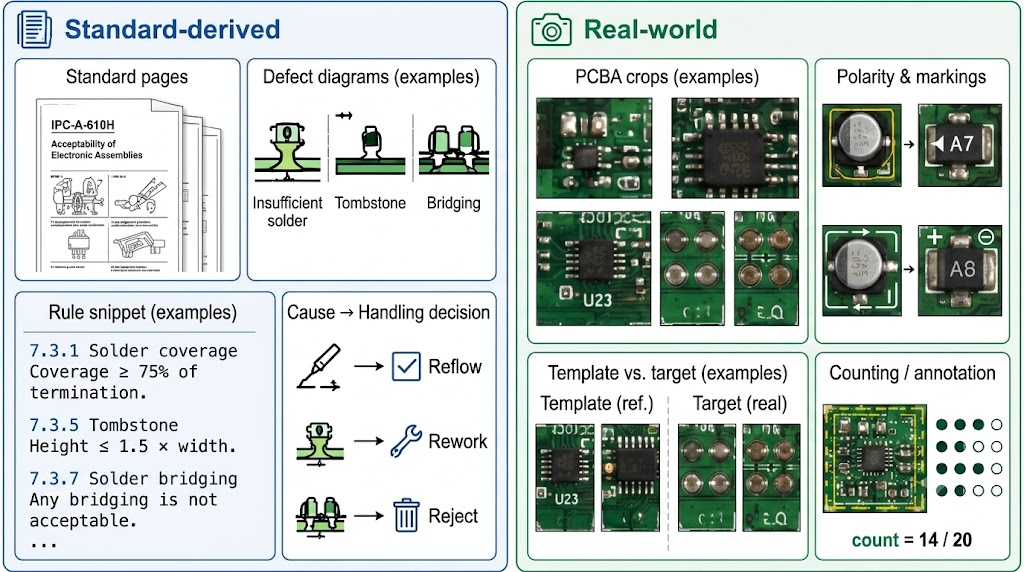
\includegraphics[width=0.91\columnwidth]{pic/pcba_data.png}
\caption{Dataset organization of the PCBA Standard-to-Real Grand Challenge. The benchmark combines standards-derived VQA for rule knowledge with real-world production-line VQA for visual inspection.}
\Description{Dataset figure showing the standard-derived and real-world PCBA VQA data organization and the corresponding task families used in the challenge.}
\label{fig:dataset}
\vspace{-1.0em}
\end{figure}

\subsection{Implementation Details}
\label{subsec:impl}

The framework is model-agnostic, but we use two Qwen3.5 model scales for different experimental purposes. All controlled ablations are conducted with Qwen3.5-9B on the fixed 8:2 training-set split, which keeps every variant under the same affordable compute budget and makes the effect of each method component easier to isolate. The final public-test submission scales the same recipe to Qwen3.5-27B and is trained on the full released training set before generating official test answers. The two teachers are initialized from the same PCBA instruction-tuned checkpoint at the corresponding scale, trained as separate LoRA adapters, and frozen during \method{} distillation. Teacher prefill uses the shared multi-LoRA serving interface described in Section~\ref{subsec:teachers}. Unless otherwise stated, the policy-gradient advantage is clipped to $A_{\max}=5$, and the final answer loss is applied only to normalized answer spans. The student is also trained parameter-efficiently in our implementation and can be merged with the base model for submission.



\begin{table}[t]
\centering
\caption{Public leaderboard.}
\vspace{-1.0em}
\label{tab:leaderboard}
\def\leaderboardscale{0.5} % Adjust this value to scale the table width.
\small
\resizebox{\leaderboardscale\columnwidth}{!}{%
\begin{tabular}{clr}
\toprule
Rank & Team & Overall \\
\midrule
1 & Ours & 90.920129 \\
2 & Team \#1 & 90.620509 \\
3 & Team \#2 & 90.542902 \\
4 & Team \#3 & 89.608524 \\
5 & Team \#4 & 88.749941 \\
\bottomrule
\end{tabular}
}
% \vspace{-0.7em}
\vspace{-1.0em}
\end{table}

\subsection{Ablation Study}
\label{subsec:ablation}

We compare \method{} with four Qwen3.5-9B variants using the fixed held-out validation split. \emph{w/o standard-domain teacher} removes the teacher specialized for standards-derived knowledge and distills only from the real-world teacher. \emph{w/o real-world teacher} removes the teacher specialized for production-line imagery and distills only from the standard-domain teacher. \emph{Direct training} trains the student directly on the 80\% ablation-training portion with the same prompt and answer format, but without domain teachers or on-policy distillation. \emph{Baseline w/o training} evaluates the shared base model without PCBA-specific post-training.

\begin{table}[t]
\centering
\caption{Qwen3.5-9B ablation results on the fixed held-out validation split. Accuracy is computed after the same answer normalization used for submission generation.}
\vspace{-1.0em}
\label{tab:ablation}
\def\ablationscale{0.6} % Adjust this value to scale the table width.
\resizebox{\ablationscale\columnwidth}{!}{%
\begin{tabular}{lc}
\toprule
Variant & Accuracy \\
\midrule
\method{} & 0.932 \\
w/o standard-domain teacher & 0.916 \\
w/o real-world teacher & 0.903 \\
direct training & 0.877 \\
baseline w/o training & 0.5573 \\
\bottomrule
\end{tabular}
}
% \vspace{-0.7em}
\vspace{-1.2em}
\end{table}


\subsection{Analysis}
\label{subsec:analysis}

The validation accuracy is higher than the official leaderboard score because the ablation validation set is sampled from the released training distribution rather than from the hidden public test labels. Even under this easier protocol, the relative ordering is informative. Full \method{} obtains the best accuracy, suggesting that the two domain teachers provide complementary supervision when distilled into a single student. Removing the standard-domain teacher causes a clear drop, which is consistent with the need for standards-derived rule knowledge in cause, handling, and defect-policy questions. Removing the real-world teacher leads to a larger drop, indicating that visual adaptation to production-line PCBA images is especially important for the held-out split.

Direct training is weaker than either single-teacher variant. This supports our main design choice: simply fitting the available training answers does not expose the student to the token-level preferences of specialized domain teachers, nor does it reduce the mismatch between the student's sampled answers and the desired normalized answer space. The baseline without PCBA-specific training is substantially lower, confirming that generic multimodal capability is not sufficient for this benchmark. Since we do not have reliable post-challenge category annotations for the official test set, we avoid per-category claims and restrict the ablation evidence to normalized held-out accuracy.

\section{Conclusion}
\label{sec:conclusion}

We presented \method, a domain-routed multi-LoRA-teacher on-policy distillation framework for the PCBA Standard-to-Real Grand Challenge. The method follows the challenge design: standards-derived examples provide rule, cause, and handling knowledge, while real-world examples provide visually diverse inspection evidence. By specializing two homologous LoRA domain teachers and distilling them through student trajectories, \method{} inherits complementary domain expertise without the instability of flat mixed training, the cost of full-checkpoint teachers, or the cost of inference-time ensembling. Controlled ablations are conducted with Qwen3.5-9B, while the final Qwen3.5-27B submission achieves 90.920129 on the official public evaluation and ranks first on the public leaderboard.

\bibliographystyle{ACM-Reference-Format}
\bibliography{main}

\end{document}
